% ============================================================
% GECW Admission Management System — Mini Project Presentation
% LaTeX Beamer | Duration: ≤ 12 minutes
% ============================================================
\documentclass[aspectratio=169, 11pt]{beamer}

% --- Theme & Colors ---
\usetheme{Madrid}
\usecolortheme{whale}

\definecolor{gecwblue}{RGB}{26, 54, 93}
\definecolor{gecwaccent}{RGB}{59, 130, 246}
\definecolor{gecwdark}{RGB}{17, 19, 24}
\definecolor{gecwgreen}{RGB}{16, 185, 129}
\definecolor{gecwred}{RGB}{239, 68, 68}
\definecolor{gecwamber}{RGB}{245, 158, 11}
\definecolor{gecwgray}{RGB}{107, 114, 128}
\definecolor{codebg}{RGB}{245, 247, 250}

\setbeamercolor{structure}{fg=gecwblue}
\setbeamercolor{title}{fg=white, bg=gecwblue}
\setbeamercolor{frametitle}{fg=white, bg=gecwblue}
\setbeamercolor{block title}{fg=white, bg=gecwaccent}
\setbeamercolor{block body}{bg=codebg}
\setbeamercolor{item}{fg=gecwaccent}
\setbeamercolor{alerted text}{fg=gecwred}
\setbeamercolor{example text}{fg=gecwgreen}

\setbeamertemplate{navigation symbols}{}
\setbeamertemplate{footline}{
    \leavevmode%
    \hbox{%
        \begin{beamercolorbox}[wd=.33\paperwidth,ht=2.5ex,dp=1ex,center]{author in head/foot}%
            \usebeamerfont{author in head/foot}\insertshortauthor
        \end{beamercolorbox}%
        \begin{beamercolorbox}[wd=.34\paperwidth,ht=2.5ex,dp=1ex,center]{title in head/foot}%
            \usebeamerfont{title in head/foot}\insertshorttitle
        \end{beamercolorbox}%
        \begin{beamercolorbox}[wd=.33\paperwidth,ht=2.5ex,dp=1ex,right]{date in head/foot}%
            \usebeamerfont{date in head/foot}\insertframenumber{} / \inserttotalframenumber\hspace*{2ex}
        \end{beamercolorbox}}%
    \vskip0pt%
}

% --- Packages ---
\usepackage[utf8]{inputenc}
\usepackage[T1]{fontenc}
\usepackage{lmodern}
\usepackage{graphicx}
\usepackage{tikz}
\usetikzlibrary{shapes.geometric, arrows.meta, positioning, fit, calc, shadows}
\usepackage{booktabs}
\usepackage{tabularx}
\usepackage{listings}
\usepackage{fontawesome5}
\usepackage{hyperref}
\usepackage{xcolor}
\usepackage{multicol}

% --- Listings Style ---
\lstset{
    basicstyle=\ttfamily\scriptsize,
    backgroundcolor=\color{codebg},
    frame=single,
    rulecolor=\color{gecwgray!30},
    keywordstyle=\color{gecwaccent}\bfseries,
    stringstyle=\color{gecwgreen},
    commentstyle=\color{gecwgray}\itshape,
    breaklines=true,
    tabsize=2,
    showstringspaces=false,
}

% --- Title Page Info ---
\title[GECW Admission System]{GECW Admission Management System}
\subtitle{A MERN Stack Web Application with Helpdesk Chatbot}
\author[Devajith P]{Devajith P}
\institute[GECW]{Government Engineering College, Wayanad\\Department of Computer Science \& Engineering}
\date{February 2026}

% ============================================================
\begin{document}

% --- SLIDE 1: Title ---
\begin{frame}[plain]
    \titlepage
\end{frame}

% --- SLIDE 2: Table of Contents ---
\begin{frame}{Outline}
    \tableofcontents
\end{frame}

% ============================================================
\section{Introduction}
% ============================================================

% --- SLIDE 3: Problem Statement ---
\begin{frame}{Problem Statement}
    \begin{columns}[T]
        \begin{column}{0.48\textwidth}
            \textbf{\color{gecwred}\faExclamationTriangle\ \ Current Challenges}
            \begin{itemize}
                \item Manual paper-based admission process
                \item Long queues for document verification
                \item No real-time status tracking for students
                \item Repetitive queries burden office staff
                \item Error-prone manual record keeping
            \end{itemize}
        \end{column}
        \begin{column}{0.48\textwidth}
            \textbf{\color{gecwgreen}\faCheckCircle\ \ Proposed Solution}
            \begin{itemize}
                \item Digital admission form (multi-step)
                \item Online document upload \& verification
                \item Real-time status tracker (dashboard)
                \item AI-powered Helpdesk Chatbot
                \item Role-based admin panel
            \end{itemize}
        \end{column}
    \end{columns}
    \vspace{0.5cm}
    \begin{block}{Technology Stack}
        \centering
        \textbf{M}ongoDB \quad $\bullet$ \quad \textbf{E}xpress.js \quad $\bullet$ \quad \textbf{R}eact.js \quad $\bullet$ \quad \textbf{N}ode.js
    \end{block}
\end{frame}

% --- SLIDE 4: System Modules ---
\begin{frame}{System Modules}
    \begin{columns}[T]
        \begin{column}{0.3\textwidth}
            \begin{block}{\faUserGraduate\ \ Student Module}
                \small
                \begin{itemize}
                    \item Registration \& Login
                    \item Multi-step admission form
                    \item Document upload
                    \item Status tracking dashboard
                    \item View admin feedback
                \end{itemize}
            \end{block}
        \end{column}
        \begin{column}{0.3\textwidth}
            \begin{block}{\faUserShield\ \ Admin Module}
                \small
                \begin{itemize}
                    \item Secure admin login
                    \item View all applications
                    \item Verify/reject documents
                    \item Update admission status
                    \item Send feedback to students
                \end{itemize}
            \end{block}
        \end{column}
        \begin{column}{0.3\textwidth}
            \begin{block}{\faRobot\ \ Chatbot Module}
                \small
                \begin{itemize}
                    \item Interactive chat interface
                    \item Keyword-based NLP matching
                    \item Knowledge base in MongoDB
                    \item Instant admission queries
                    \item Fallback responses
                \end{itemize}
            \end{block}
        \end{column}
    \end{columns}
\end{frame}

% ============================================================
\section{Data Flow Diagrams}
% ============================================================

% --- SLIDE 5: Context Level DFD (Level 0) ---
\begin{frame}{DFD — Level 0 (Context Diagram)}
    \centering
    \begin{tikzpicture}[
        node distance=3.5cm,
        entity/.style={rectangle, draw=gecwblue, fill=gecwblue!10, thick, minimum width=2.8cm, minimum height=1cm, font=\small\bfseries, rounded corners=3pt},
        process/.style={circle, draw=gecwaccent, fill=gecwaccent!15, thick, minimum size=2.5cm, font=\small\bfseries, text width=2.2cm, align=center},
        arrow/.style={-{Stealth[length=3mm]}, thick, gecwdark},
    ]
        % Entities
        \node[entity] (student) at (-5, 0) {\faUserGraduate\ Student};
        \node[entity] (admin)   at ( 5, 0) {\faUserShield\ Admin};

        % Central process
        \node[process] (system) at (0, 0) {Admission Management System};

        % Arrows: Student <-> System
        \draw[arrow] (student.north east) -- node[above, font=\scriptsize, text=gecwgray]{Registration, Form, Documents} (system.north west);
        \draw[arrow] (system.south west) -- node[below, font=\scriptsize, text=gecwgray]{Status, Feedback, Chatbot Response} (student.south east);

        % Arrows: System <-> Admin
        \draw[arrow] (system.north east) -- node[above, font=\scriptsize, text=gecwgray]{Student Data, Documents} (admin.north west);
        \draw[arrow] (admin.south west) -- node[below, font=\scriptsize, text=gecwgray]{Verify, Reject, Remarks} (system.south east);

        % Database
        \node[rectangle, draw=gecwdark, fill=gecwdark!10, thick, minimum width=2.5cm, minimum height=0.8cm, font=\small\bfseries, rounded corners=2pt] (db) at (0, -2.8) {\faDatabase\ MongoDB Atlas};
        \draw[arrow, <->] (system.south) -- node[right, font=\scriptsize, text=gecwgray]{CRUD Operations} (db.north);
    \end{tikzpicture}
\end{frame}

% --- SLIDE 6: Level 1 DFD ---
\begin{frame}{DFD — Level 1 (Detailed Data Flow)}
    \centering
    \begin{tikzpicture}[
        node distance=1.8cm,
        process/.style={circle, draw=gecwaccent, fill=gecwaccent!10, thick, minimum size=1.3cm, font=\tiny\bfseries, text width=1.1cm, align=center},
        store/.style={rectangle, draw=gecwdark, fill=gecwdark!5, thick, minimum width=2cm, minimum height=0.6cm, font=\tiny\bfseries, rounded corners=2pt},
        entity/.style={rectangle, draw=gecwblue, fill=gecwblue!10, thick, minimum width=1.8cm, minimum height=0.6cm, font=\tiny\bfseries, rounded corners=2pt},
        arrow/.style={-{Stealth[length=2mm]}, thick, gecwdark!70},
        label/.style={font=\tiny, text=gecwgray},
        scale=0.95
    ]
        % External Entities
        \node[entity] (student) at (-6, 0.5) {\faUser\ Student};
        \node[entity] (admin)   at ( 6, 0.5) {\faUserCog\ Admin};

        % Processes
        \node[process] (p1) at (-3.2, 1.8) {1.0\\Auth};
        \node[process] (p2) at (-0.5, 1.8) {2.0\\Form\\Submit};
        \node[process] (p3) at ( 2.2, 1.8) {3.0\\Doc\\Upload};
        \node[process] (p4) at ( 4.5, 0.5) {4.0\\Verify\\Docs};
        \node[process] (p5) at (-3.2,-1.5) {5.0\\Chatbot\\Query};

        % Data Stores
        \node[store] (ds1) at (-0.5, -0.8) {\faDatabase\ D1: Students};
        \node[store] (ds2) at ( 2.2, -0.8) {\faDatabase\ D2: Uploads};
        \node[store] (ds3) at (-3.2, -3.2) {\faDatabase\ D3: KnowledgeBase};
        \node[store] (ds4) at ( 4.5, -1.5) {\faDatabase\ D4: Admins};

        % Student -> Auth
        \draw[arrow] (student) |- node[label, above left]{Credentials} (p1);
        % Auth -> Student DB
        \draw[arrow] (p1) -- node[label, right]{Save/Verify} (ds1);
        % Auth -> Student (token)
        \draw[arrow, gecwgreen!70!black] (p1) -- node[label, left]{JWT Token} (student);

        % Student -> Form
        \draw[arrow] (student) |- node[label, above]{Form Data} ([yshift=5pt]p2.west);
        % Form -> Student DB
        \draw[arrow] (p2) -- node[label, right]{Update Profile} (ds1);

        % Student -> Upload
        \draw[arrow] (student.north) |- node[label, above]{Files} ([yshift=5pt]p3.west);
        % Upload -> File Store
        \draw[arrow] (p3) -- node[label, right]{Save File} (ds2);
        % Upload -> Student DB
        \draw[arrow] (p3.south west) -- node[label, below left]{Doc Ref} (ds1.east);

        % Admin -> Verify
        \draw[arrow] (admin) -- node[label, right]{Review} (p4);
        % Verify <-> Student DB
        \draw[arrow] (p4) -- node[label, right]{Status Update} (ds4);
        \draw[arrow, <->] (ds1.east) -| node[label, below]{Read/Write} (p4.south);

        % Student -> Chatbot
        \draw[arrow] (student) |- node[label, left]{Query} (p5);
        % Chatbot -> KB
        \draw[arrow, <->] (p5) -- node[label, right]{Match} (ds3);
        % Chatbot -> Student (response)
        \draw[arrow, gecwgreen!70!black, dashed] (p5.west) -| node[label, below left]{Answer} ([yshift=-5pt]student.south);
    \end{tikzpicture}
\end{frame}

% --- SLIDE 7: Level 2 DFD (Student Auth) ---
\begin{frame}{DFD — Level 2 (Authentication Process)}
    \centering
    \begin{tikzpicture}[
        node distance=2cm,
        process/.style={circle, draw=gecwaccent, fill=gecwaccent!10, thick, minimum size=1.5cm, font=\scriptsize\bfseries, text width=1.3cm, align=center},
        store/.style={rectangle, draw=gecwdark, fill=gecwdark!5, thick, minimum width=2.5cm, minimum height=0.7cm, font=\scriptsize\bfseries, rounded corners=2pt},
        entity/.style={rectangle, draw=gecwblue, fill=gecwblue!10, thick, minimum width=2cm, minimum height=0.8cm, font=\scriptsize\bfseries, rounded corners=2pt},
        arrow/.style={-{Stealth[length=2.5mm]}, thick, gecwdark!70},
        label/.style={font=\tiny, text=gecwgray},
    ]
        \node[entity] (user) at (-5, 0) {\faUser\ User};

        \node[process] (p1) at (-2, 1.5) {1.1\\Validate\\Input};
        \node[process] (p2) at ( 1, 1.5) {1.2\\Hash\\Password};
        \node[process] (p3) at ( 4, 1.5) {1.3\\Save to\\Database};
        \node[process] (p4) at (-2,-1.5) {1.4\\Verify\\Credentials};
        \node[process] (p5) at ( 1,-1.5) {1.5\\Generate\\JWT};
        \node[process] (p6) at ( 4,-1.5) {1.6\\Return\\Token};

        \node[store] (db) at (4, 0) {\faDatabase\ Student Collection};

        % Registration flow (top)
        \node[font=\scriptsize\bfseries, text=gecwaccent] at (-0.5, 2.5) {Registration Flow};
        \draw[arrow] (user.north east) -- node[label, above]{App No + Password} (p1);
        \draw[arrow] (p1) -- node[label, above]{Valid Data} (p2);
        \draw[arrow] (p2) -- node[label, above]{bcrypt Hash} (p3);
        \draw[arrow] (p3) -- node[label, right]{Insert} (db);

        % Login flow (bottom)
        \node[font=\scriptsize\bfseries, text=gecwgreen] at (-0.5, -2.5) {Login Flow};
        \draw[arrow] (user.south east) -- node[label, below]{Credentials} (p4);
        \draw[arrow, <->] (p4) -- node[label, left]{Lookup} (db);
        \draw[arrow] (p4) -- node[label, below]{bcrypt Compare} (p5);
        \draw[arrow] (p5) -- node[label, below]{JWT} (p6);
        \draw[arrow, gecwgreen, dashed] (p6.south) -- ++(0,-0.7) -| node[label, below]{Token Response} (user.south);
    \end{tikzpicture}
\end{frame}

% ============================================================
\section{Database Design}
% ============================================================

% --- SLIDE 8: ER Diagram ---
\begin{frame}{Database Design — Entity Relationship Diagram}
    \centering
    \begin{tikzpicture}[
        entity/.style={rectangle, draw=gecwblue, fill=gecwblue!8, thick, minimum width=3cm, minimum height=0.8cm, font=\small\bfseries, rounded corners=3pt},
        attr/.style={font=\tiny, text=gecwdark, align=left},
        rel/.style={diamond, draw=gecwaccent, fill=gecwaccent!15, thick, aspect=2.5, font=\tiny\bfseries, inner sep=1pt},
        arrow/.style={-{Stealth[length=2mm]}, thick, gecwdark!60},
        scale=0.92, transform shape
    ]
        % Student Entity
        \node[entity] (student) at (0, 0) {\faUserGraduate\ Student};
        \node[attr, below=0.3cm of student, text width=4cm] (sattr) {
            \underline{\_id} : ObjectId (PK)\\
            keamAppNumber : String (Unique)\\
            password : String (Hashed)\\
            personalDetails : \{name, email, phone, dob, address\}\\
            guardianDetails : \{name, relation, phone\}\\
            academicDetails : \{keamRank, rollNo, marks, school\}\\
            category : Enum [General, SC, ST, OEC, SEBC]\\
            branch : Enum [CSE, ECE, EEE, ME, CE]\\
            status : Enum [Submitted, Verified, Admitted, ...]\\
            adminRemarks : String\\
            createdAt : Date
        };

        % Documents (embedded)
        \node[entity] (docs) at (7, 0) {\faFileAlt\ Documents[ ]};
        \node[attr, below=0.3cm of docs, text width=3cm] (dattr) {
            \underline{\_id} : ObjectId\\
            name : String\\
            url : String (file path)\\
            status : Enum [Pending, Verified, Rejected]\\
            adminFeedback : String
        };

        % Admin Entity
        \node[entity] (admin) at (0, -5.5) {\faUserShield\ Admin};
        \node[attr, below=0.3cm of admin, text width=3.5cm] (aattr) {
            \underline{\_id} : ObjectId (PK)\\
            username : String (Unique)\\
            password : String (Hashed)\\
            role : Enum [Clerk, HOD, Principal]\\
            branch : Enum [CSE, ..., All]\\
            createdAt : Date
        };

        % KnowledgeBase Entity
        \node[entity] (kb) at (7, -5.5) {\faRobot\ KnowledgeBase};
        \node[attr, below=0.3cm of kb, text width=3cm] (kattr) {
            \underline{\_id} : ObjectId (PK)\\
            keywords : [String]\\
            answer : String\\
            category : Enum [Fees, Hostel, ...]
        };

        % Relationships
        \node[rel] (r1) at (3.5, 0) {embeds};
        \draw[arrow] (student) -- (r1);
        \draw[arrow] (r1) -- (docs);
        \node[font=\tiny, text=gecwgray] at (3.5, 0.5) {1 : N};

        \node[rel] (r2) at (0, -3.5) {verifies};
        \draw[arrow] (admin) -- (r2);
        \draw[arrow] (r2) -- (student);
        \node[font=\tiny, text=gecwgray] at (0.7, -3.5) {1 : N};

        \node[rel] (r3) at (7, -3.5) {queries};
        \draw[arrow, dashed] ([xshift=20pt]student.south east) |- (r3);
        \draw[arrow] (r3) -- (kb);
        \node[font=\tiny, text=gecwgray] at (7.7, -3.5) {N : N};
    \end{tikzpicture}
\end{frame}

% --- SLIDE 9: Schema Details ---
\begin{frame}{Database Design — MongoDB Schema}
    \begin{columns}[T]
        \begin{column}{0.48\textwidth}
            \begin{block}{Student Schema (Mongoose)}
                \lstinputlisting[language=Java, firstline=1, lastline=12, basicstyle=\ttfamily\tiny]{%
                    dummy_schema.txt%
                }
            \end{block}
            % Since lstinputlisting won't work, use lstlisting instead
            \vspace{-0.5cm}
            \begin{lstlisting}[language=Java, basicstyle=\ttfamily\tiny]
StudentSchema = {
  keamAppNumber: String (unique),
  password:      String (hashed),
  personalDetails: {
    name, email, phone, dob, address
  },
  guardianDetails: {
    name, relation, phone
  },
  academicDetails: {
    keamRank, keamRollNo,
    plusTwoMarks, schoolName
  },
  documents: [{ name, url,
    status, adminFeedback }],
  status: Enum,
  adminRemarks: String
}
            \end{lstlisting}
        \end{column}
        \begin{column}{0.48\textwidth}
            \begin{block}{Admin Schema}
            \end{block}
            \vspace{-0.3cm}
            \begin{lstlisting}[language=Java, basicstyle=\ttfamily\tiny]
AdminSchema = {
  username: String (unique),
  password: String (hashed),
  role:     Enum [Admission Clerk,
                  HOD, Principal],
  branch:   Enum [CSE, ECE, EEE,
                  ME, CE, All]
}
            \end{lstlisting}

            \begin{block}{KnowledgeBase Schema}
            \end{block}
            \vspace{-0.3cm}
            \begin{lstlisting}[language=Java, basicstyle=\ttfamily\tiny]
KnowledgeBaseSchema = {
  keywords: [String] (lowercase),
  answer:   String (required),
  category: Enum [Fees, Hostel,
                  Transport, General]
}
            \end{lstlisting}

            \vspace{0.3cm}
            \begin{alertblock}{\footnotesize Key Design Decisions}
                \tiny
                \begin{itemize}
                    \item Documents are \textbf{embedded} (not referenced) for atomic reads
                    \item Passwords hashed with \textbf{bcrypt} (never stored in plain text)
                    \item Admin seeded automatically on server startup
                \end{itemize}
            \end{alertblock}
        \end{column}
    \end{columns}
\end{frame}

% ============================================================
\section{UI Design}
% ============================================================

% --- SLIDE 10: UI - Component Architecture ---
\begin{frame}{UI Design — Component Architecture}
    \centering
    \begin{tikzpicture}[
        comp/.style={rectangle, draw=gecwaccent, fill=gecwaccent!8, thick, minimum width=2.8cm, minimum height=0.8cm, font=\scriptsize\bfseries, rounded corners=5pt},
        page/.style={rectangle, draw=gecwblue, fill=gecwblue!8, thick, minimum width=2.5cm, minimum height=0.7cm, font=\scriptsize\bfseries, rounded corners=5pt},
        svc/.style={rectangle, draw=gecwgreen!70!black, fill=gecwgreen!8, thick, minimum width=2.5cm, minimum height=0.7cm, font=\scriptsize\bfseries, rounded corners=5pt},
        arrow/.style={-{Stealth[length=2mm]}, thick, gecwdark!50},
        scale=0.85, transform shape
    ]
        % App.jsx (root)
        \node[comp, minimum width=12cm, fill=gecwdark!8, draw=gecwdark] (app) at (0, 3.5) {\faReact\ App.jsx (HashRouter + Routes)};

        % Shared Components
        \node[comp] (navbar) at (-4, 2.2) {\faCompass\ Navbar.jsx};
        \node[comp] (footer) at ( 4, 2.2) {\faGripLines\ Footer.jsx};

        % Pages
        \node[page] (home)    at (-5, 0.8) {Home.jsx};
        \node[page] (auth)    at (-2.5, 0.8) {Auth.jsx};
        \node[page] (form)    at ( 0, 0.8) {AdmissionForm.jsx};
        \node[page] (upload)  at ( 2.8, 0.8) {DocumentUpload.jsx};
        \node[page] (sdash)   at (-3.5, -0.5) {StudentDashboard.jsx};
        \node[page] (adash)   at ( 0, -0.5) {AdminDashboard.jsx};
        \node[page] (chat)    at ( 3.5, -0.5) {Chatbot.jsx};

        % Services
        \node[svc] (api) at (0, -2) {\faPlug\ api.js (Axios + JWT Interceptor)};
        \node[svc, draw=gecwamber, fill=gecwamber!8] (ls) at (0, -3) {\faKey\ localStorage (token, user, admin)};

        % Routes from App
        \draw[arrow] (app) -- (navbar);
        \draw[arrow] (app) -- (footer);
        \draw[arrow] (app.south) -- ++(0,-0.1) -| (home);
        \draw[arrow] (app.south) -- ++(0,-0.1) -| (auth);
        \draw[arrow] (app.south) -- ++(0,-0.1) -| (form);
        \draw[arrow] (app.south) -- ++(0,-0.1) -| (upload);

        % Pages -> API service
        \draw[arrow, dashed, gecwgreen!70!black] (sdash) -- (api);
        \draw[arrow, dashed, gecwgreen!70!black] (adash) -- (api);
        \draw[arrow, dashed, gecwgreen!70!black] (chat) -- (api);
        \draw[arrow, dashed, gecwgreen!70!black] (auth.south) -- ++(0,-0.3) -| (api);

        % API -> localStorage
        \draw[arrow, gecwamber] (api) -- (ls);

        % Route labels
        \node[font=\tiny, text=gecwgray] at (-5, 1.3) {/};
        \node[font=\tiny, text=gecwgray] at (-2.5, 1.3) {/login, /register};
        \node[font=\tiny, text=gecwgray] at (0, 1.3) {/apply};
        \node[font=\tiny, text=gecwgray] at (2.8, 1.3) {/upload};
        \node[font=\tiny, text=gecwgray] at (-3.5, -0.05) {/dashboard};
        \node[font=\tiny, text=gecwgray] at (0, -0.05) {/admin/dashboard};
        \node[font=\tiny, text=gecwgray] at (3.5, -0.05) {/chat};
    \end{tikzpicture}
\end{frame}

% --- SLIDE 11: UI - Key Screens ---
\begin{frame}{UI Design — Key Screens}
    \begin{columns}[T]
        \begin{column}{0.48\textwidth}
            \textbf{\color{gecwaccent}\faDesktop\ Student-Facing Screens}
            \vspace{0.2cm}

            \begin{block}{\scriptsize 1. Home Page}
                \tiny Hero section with college branding, call-to-action buttons for Login/Register, feature highlights, animated entrance with Framer Motion.
            \end{block}

            \begin{block}{\scriptsize 2. Authentication (Login / Register)}
                \tiny Centered card with KEAM App Number field, password field, icon-prefixed inputs, toggle between Login and Register modes, admin login variant. Error displayed in red alert box.
            \end{block}

            \begin{block}{\scriptsize 3. Multi-Step Admission Form}
                \tiny 3-step wizard — Personal $\rightarrow$ Guardian $\rightarrow$ Academic. Step indicator at top, form validation, data saved via PUT request.
            \end{block}

            \begin{block}{\scriptsize 4. Document Upload}
                \tiny Drag-and-drop file input. Lists uploaded docs with status badges (Pending/Verified/Rejected). 5MB limit, PDF/JPG/PNG only.
            \end{block}
        \end{column}

        \begin{column}{0.48\textwidth}
            \textbf{\color{gecwblue}\faUserCog\ Admin \& Chatbot Screens}
            \vspace{0.2cm}

            \begin{block}{\scriptsize 5. Student Dashboard}
                \tiny Progress tracker (Form Filled $\rightarrow$ Verified $\rightarrow$ Admitted). Quick action cards. Admin feedback section in red. Rejected docs listed with re-upload link.
            \end{block}

            \begin{block}{\scriptsize 6. Admin Dashboard}
                \tiny Stat cards (Total, Verified, Submitted, Admitted). Branch seat tracker with progress bars. Filterable student table. Full-screen review modal with document viewer, approve/reject buttons, and feedback textarea.
            \end{block}

            \begin{block}{\scriptsize 7. Helpdesk Chatbot}
                \tiny Chat bubble interface. Bot messages left-aligned, user messages right-aligned. Typing indicator animation. Auto-scroll. Powered by keyword-matching NLP.
            \end{block}

            \vspace{0.2cm}
            \begin{exampleblock}{\scriptsize Design Principles}
                \tiny Modern glassmorphism, rounded corners (3xl), primary blue theme, Framer Motion animations, Material Symbols icons, fully responsive.
            \end{exampleblock}
        \end{column}
    \end{columns}
\end{frame}

% --- SLIDE 12: UI Flow Diagram ---
\begin{frame}{UI Design — User Navigation Flow}
    \centering
    \begin{tikzpicture}[
        screen/.style={rectangle, draw=gecwaccent, fill=white, thick, minimum width=2.2cm, minimum height=1cm, font=\tiny\bfseries, rounded corners=5pt, drop shadow={shadow xshift=1pt, shadow yshift=-1pt, opacity=0.15}},
        arrow/.style={-{Stealth[length=2mm]}, thick, gecwaccent!70},
        note/.style={font=\tiny, text=gecwgray, align=center},
        scale=0.9, transform shape
    ]
        % Student Flow
        \node[font=\scriptsize\bfseries, text=gecwblue] at (-5, 2.5) {Student Flow};

        \node[screen] (home) at (-5, 1.2) {\faHome\\Home};
        \node[screen] (reg)  at (-2.5, 1.2) {\faUserPlus\\Register};
        \node[screen] (login) at (-2.5, -0.5) {\faSignInAlt\\Login};
        \node[screen, fill=gecwaccent!5] (dash) at (0.5, 0.3) {\faTachometerAlt\\Dashboard};
        \node[screen] (form) at (3, 1.5) {\faWpforms\\Admission\\Form};
        \node[screen] (upl) at (3, -0.8) {\faUpload\\Document\\Upload};
        \node[screen] (bot) at (0.5, -1.8) {\faRobot\\Chatbot};

        \draw[arrow] (home) -- (reg);
        \draw[arrow] (home) -- (login);
        \draw[arrow] (reg) -- node[note, right]{JWT} (dash);
        \draw[arrow] (login) -- node[note, right]{JWT} (dash);
        \draw[arrow] (dash) -- (form);
        \draw[arrow] (dash) -- (upl);
        \draw[arrow] (dash) -- (bot);

        % Admin Flow
        \node[font=\scriptsize\bfseries, text=gecwblue] at (-5, -2.5) {Admin Flow};

        \node[screen, fill=gecwblue!5] (alogin) at (-5, -3.8) {\faLock\\Admin\\Login};
        \node[screen, fill=gecwblue!5, minimum width=3.5cm] (adash)  at (-1, -3.8) {\faClipboardList\\Admin Dashboard\\(Table + Stats)};
        \node[screen, fill=gecwblue!5, minimum width=3cm] (review) at (3, -3.8) {\faSearchPlus\\Review Modal\\(Docs + Verify)};

        \draw[arrow] (home) |- (alogin);
        \draw[arrow, gecwblue] (alogin) -- node[note, above]{JWT} (adash);
        \draw[arrow, gecwblue] (adash) -- node[note, above]{Click} (review);

        % Navbar
        \node[rectangle, draw=gecwdark, fill=gecwdark!5, thick, minimum width=12cm, minimum height=0.5cm, font=\tiny\bfseries, rounded corners=2pt] at (-0.5, 3.2) {\faCompass\ Navbar (persistent) — Logo | Helpdesk | \faEllipsisV\ Menu (Home, Dashboard, Form, Upload, Logout)};
    \end{tikzpicture}
\end{frame}

% ============================================================
\section{GitHub Commit History}
% ============================================================

% --- SLIDE 13: Commit History ---
\begin{frame}{GitHub Commit History}
    \begin{columns}[T]
        \begin{column}{0.55\textwidth}
            \footnotesize
            \textbf{\faGithub\ Repository:} \href{https://github.com/Devajith11/COLLEGE-ADMISSION-MANAGEMENT-SYSTEM}{Devajith11/COLLEGE-ADMISSION-MANAGEMENT-SYSTEM}\\
            \textbf{Total Commits:} 21 \quad \textbf{Branch:} main
            \vspace{0.3cm}

            \tiny
            \begin{tabular}{@{}p{0.8cm} p{5.5cm}@{}}
                \toprule
                \textbf{Hash} & \textbf{Commit Message} \\
                \midrule
                \texttt{4f0f9ab} & Initial commit \\
                \texttt{e74fff1} & Setup .gitignore and remove tracked dependencies \\
                \texttt{6acd363} & Cleanup: remove tracked uploads and secrets \\
                \texttt{d3a14fb} & Clean up uploaded files, restructure uploads \\
                \texttt{a8cd51a} & Add .nojekyll to bypass Jekyll build \\
                \texttt{6add19e} & Add \_config.yml for Jekyll exclusion \\
                \texttt{3bfb5d2} & Configure Vite base path \& GitHub Actions \\
                \texttt{b2d0d0b} & Use HashRouter for GitHub Pages routing \\
                \texttt{3845ec0} & Improve error handling, auto-seed admin \\
                \texttt{7b589d6} & Update API URL to Render backend \\
                \texttt{3b3de07} & Use navigate() to avoid GH Pages 404 \\
                \bottomrule
            \end{tabular}
        \end{column}
        \begin{column}{0.42\textwidth}
            \tiny
            \begin{tabular}{@{}p{0.8cm} p{4cm}@{}}
                \toprule
                \textbf{Hash} & \textbf{Commit Message} \\
                \midrule
                \texttt{95bdf24} & Improve document viewing \& admin token \\
                \texttt{666b3e3} & Improve admin doc preview with iframe \\
                \texttt{42c17ab} & Ensure admin credentials on startup \\
                \texttt{cb8d528} & Connect to DB before seeding admin \\
                \texttt{804180f} & Add debug endpoint \& error logging \\
                \texttt{1af9789} & Add root welcome route to backend \\
                \texttt{a130f83} & Display full student details in admin \\
                \texttt{026d9ab} & Enhance admin UI visibility \& aesthetics \\
                \texttt{82909a7} & Add admin-student feedback system \\
                \texttt{d9cdca2} & Fix navbar: dropdown menu + logout \\
                \bottomrule
            \end{tabular}

            \vspace{0.3cm}
            \begin{exampleblock}{\scriptsize Commit Categories}
                \tiny
                \begin{itemize}
                    \item \textbf{feat:} New features (6 commits)
                    \item \textbf{fix:} Bug fixes (5 commits)
                    \item \textbf{chore:} Maintenance (5 commits)
                    \item \textbf{build/design:} Config \& UI (5 commits)
                \end{itemize}
            \end{exampleblock}
        \end{column}
    \end{columns}
\end{frame}

% --- SLIDE 14: Deployment Architecture ---
\begin{frame}{Deployment Architecture}
    \centering
    \begin{tikzpicture}[
        box/.style={rectangle, draw=#1, fill=#1!8, thick, minimum width=3.5cm, minimum height=1.5cm, font=\small\bfseries, rounded corners=8pt, text width=3.2cm, align=center},
        arrow/.style={-{Stealth[length=3mm]}, ultra thick, gecwdark!40},
        note/.style={font=\tiny, text=gecwgray, align=center},
        scale=0.85, transform shape
    ]
        % Developer
        \node[box=gecwdark] (dev) at (-6, 0) {\faLaptopCode\\Developer\\(Local Machine)};

        % GitHub
        \node[box=gecwdark!80!white] (gh) at (-1, 0) {\faGithub\\GitHub Repo\\(Source Code)};

        % GitHub Actions
        \node[box=gecwaccent] (ga) at (-1, -3) {\faCogs\\GitHub Actions\\(CI/CD Pipeline)};

        % GitHub Pages
        \node[box=gecwgreen!70!black] (gp) at (4, -3) {\faGlobe\\GitHub Pages\\(Frontend Host)};

        % Render
        \node[box=gecwblue] (render) at (4, 0) {\faServer\\Render.com\\(Backend API)};

        % MongoDB Atlas
        \node[box=gecwamber] (mongo) at (4, 3) {\faDatabase\\MongoDB Atlas\\(Cloud Database)};

        % Arrows
        \draw[arrow] (dev) -- node[note, above]{\texttt{git push}} (gh);
        \draw[arrow] (gh) -- node[note, left]{Triggers\\on push} (ga);
        \draw[arrow] (ga) -- node[note, above]{\texttt{npm build}\\Deploy dist/} (gp);
        \draw[arrow] (gh.east) -- node[note, above]{Auto\\Deploy} (render.west);
        \draw[arrow, <->] (render) -- node[note, right]{Mongoose\\Connection} (mongo);
        \draw[arrow, dashed, gecwgreen!70!black] (gp.north east) -- node[note, right, xshift=5pt]{API Calls\\(HTTPS)} (render.south);

        % URLs
        \node[font=\tiny\ttfamily, text=gecwgreen!70!black] at (4, -4.5) {devajith11.github.io/COLLEGE-ADMISSION-MANAGEMENT-SYSTEM};
        \node[font=\tiny\ttfamily, text=gecwblue] at (4, -1) {college-admission-management-system.onrender.com};
    \end{tikzpicture}
\end{frame}

% ============================================================
\section{Conclusion}
% ============================================================

% --- SLIDE 15: Conclusion ---
\begin{frame}{Conclusion \& Future Scope}
    \begin{columns}[T]
        \begin{column}{0.48\textwidth}
            \textbf{\color{gecwaccent}\faCheckDouble\ \ What We Built}
            \begin{itemize}
                \item Full-stack MERN admission portal
                \item JWT-based secure authentication
                \item Multi-step form with file uploads
                \item Admin panel with document verification
                \item Helpdesk chatbot with NLP matching
                \item CI/CD deployment pipeline
            \end{itemize}
            \vspace{0.3cm}
            \begin{block}{Key Outcomes}
                \small
                \begin{itemize}
                    \item Reduced manual paperwork
                    \item Real-time status tracking
                    \item 24/7 query resolution via chatbot
                    \item Transparent admission process
                \end{itemize}
            \end{block}
        \end{column}
        \begin{column}{0.48\textwidth}
            \textbf{\color{gecwblue}\faRocket\ \ Future Scope}
            \begin{itemize}
                \item Email/SMS notifications on status change
                \item Payment gateway integration (fees)
                \item Advanced NLP chatbot (LLM-based)
                \item PDF generation of admission receipt
                \item Analytics dashboard for admin
                \item Mobile app (React Native)
                \item Multi-college support
            \end{itemize}
            \vspace{0.3cm}
            \begin{alertblock}{\footnotesize Limitations}
                \small
                \begin{itemize}
                    \item Chatbot uses keyword matching (not deep NLP)
                    \item No email verification on registration
                    \item Single-server deployment
                \end{itemize}
            \end{alertblock}
        \end{column}
    \end{columns}
\end{frame}

% --- SLIDE 16: Thank You ---
\begin{frame}[plain]
    \centering
    \vspace{1.5cm}
    {\Huge\bfseries\color{gecwblue} Thank You!}
    \vspace{0.5cm}

    {\large\color{gecwgray} Questions?}
    \vspace{1cm}

    \begin{tikzpicture}
        \node[rectangle, draw=gecwaccent, fill=gecwaccent!5, thick, rounded corners=10pt, minimum width=8cm, minimum height=2cm, font=\small] {
            \begin{tabular}{rl}
                \faUser & \textbf{Devajith P} \\
                \faUniversity & Government Engineering College, Wayanad \\
                \faGithub & \href{https://github.com/Devajith11/COLLEGE-ADMISSION-MANAGEMENT-SYSTEM}{github.com/Devajith11/COLLEGE-ADMISSION-MANAGEMENT-SYSTEM} \\
                \faGlobe & \href{https://devajith11.github.io/COLLEGE-ADMISSION-MANAGEMENT-SYSTEM/}{devajith11.github.io/COLLEGE-ADMISSION-MANAGEMENT-SYSTEM} \\
            \end{tabular}
        };
    \end{tikzpicture}
\end{frame}

\end{document}
